\chapter{Implementation}
\label{ch:implementation}

In this chapter, we discuss in detail the construction of the synchronized hybrid editor. Our implementation comes on top of the already existing TurtleEditor \cite{Petersen2016} so we start with presenting its features. Then, we explain the high-level architecture and, finally, we provide a step-by-step description of the implemented modules.


\section {Preliminaries}
\label{sec:preliminaries}

The code editing requirement has been already fulfilled by the TurtleEditor project, implemented in Javascript. This is an open-source web client which incorporates a code editor supporting features like syntax highlighting, syntax checking and auto-completion. Besides this, communication with external sources can also be realized by loading files from and committing changes to a central repository \cite{Petersen2016}.

The following is a list of features the TurtleEditor comes with and that will be, as well, part of our final application:

\begin{itemize}
	\item \textbf{code editing}: implemented using the \textit{CodeMirror}\footnote{\url{https://codemirror.net}} Javascript library, which also supports syntax highlighting for more than 100 languages, including Turtle - the language that our hybrid editor will use in its code view for designing vocabularies.
	\item \textbf{auto completion}: realized with CodeMirror as well, with the help of its add-on \textit{hint}, which requires defining the namespaces internally. Once a certain event is triggered (a keyboard combination, in our case - \textit{Ctrl}+\textit{Space}), the look-up process is started and, if the namespace is found (i.e., it was previously defined), a list of available terms will be displayed in order to choose from.
	\item \textbf{validation}: implemented using the \textit{N3.js}\footnote{\url{https://github.com/RubenVerborgh/N3.js}} Javascript library, which supports parsing Turtle code and detects possible syntax errors. Once this occurs, the faulty line is highlighted in red and a tooltip with additional information is provided via a red dot placed besides the line number.
	\item \textbf{repository communication}: realized by using the REST interface provided by the GitHub repository. The user can input a repository source that will be checked out and a dropdown menu will be populated with the available vocabulary files so that they can be browsed and selected for editing.
	\item \textbf{access control}: this feature is needed for accessing and writing to private repositories. The user can log in with credentials or by using a generated personal access token to authenticate with the GitHub REST API \cite{Petersen2016}.
\end{itemize}


\section {Architecture}

\autoref{img:turtle_architecture} shows the high-level architecture of the TurtleEditor. The project basically consists of a web client supporting the features presented in the previous section. Since repository communication is also included, the diagram displays the server side too, which actually represents the repository hosting service together with the services that it is supposed to provide: access control, issue tracking, a wiki for the documentation and the version-controlled repository itself.

Our hybrid editor is entirely developed on the client side and it represents an enhancement of the web client. On top of the features supported by the TurtleEditor, we add the implementation of the requirements presented in \autoref{ch:requirements}: graphical editing, synchronization of the two editors and the visualization module which includes various functionalities for displaying RDF data in a meaningful way. The enhanced client, which represents our contribution, is displayed in \autoref{img:client}

\begin{figure}[!htbp]
	\centering
  	\centerline{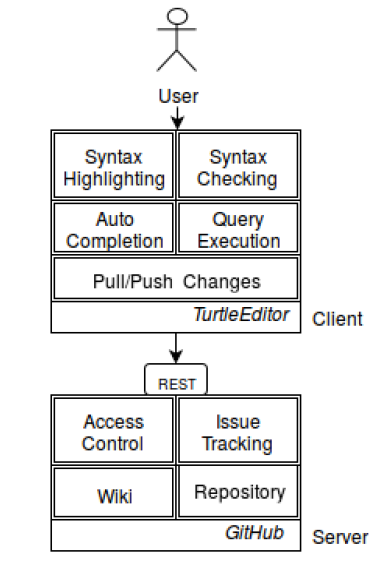
\includegraphics[height=11cm]{img/turtleeditor_architecture.png}}
	\caption{TurtleEditor architecture. Figure taken from \cite{Petersen2016}.}
	\label{img:turtle_architecture}
\end{figure}

\begin{figure}[!htbp]
	\centering
  	\centerline{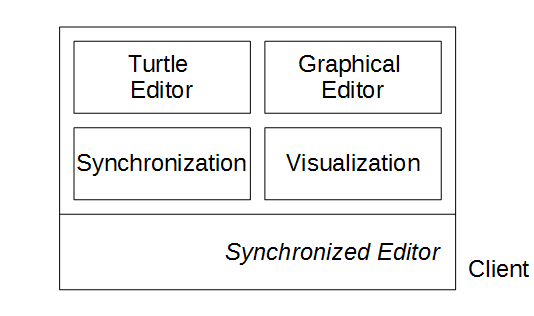
\includegraphics[height=5cm]{img/client.png}}
	\caption{Enhanced client.}
	\label{img:client}
\end{figure}


\section {Modules}

The synchronized hybrid editor is implemented in Javascript and can be run using a web browser. A few Javascript libraries, such as \textit{JQuery}\footnote{\url{https://jquery.com}}, \textit{vis.js}\footnote{\url{http://visjs.org}} and \textit{split-pane.js}\footnote{\url{https://github.com/shagstrom/split-pane}}, are employed in developing certain functionalities. The role each of these libraries plays in our implementation is discussed in detail in what follows. The remainder of this section explains how the requirements listed in \autoref{ch:requirements} have been approached.

\subsection {Graphical Editing}
\label{subsec:graphical_editing}

The concepts defined using Turtle code are basically interrelated entities so the apparent structure that can be employed in any graphical functionality is a graph or, in other words, a network. One mature Javascript library that supports manipulating such a structure is \textit{vis.js}. It is an open-source project licensed under Apache 2.0 and MIT and its first working version was released in 2013, since then being constantly upgraded. Our implementation uses version 4.16.1, released in April 2016. 

Currently, \textit{vis.js} consists of five components that enable data manipulation and interaction: DataSet, Timeline, Network, Graph2d and Graph3d. We are going to make use of the Network component in conjunction with the DataSet, which was designed to easily handle large amounts of dynamic data. The Network assures the realization of all the graphical functionalities of the editor as it supports a high degree of visual customization and comes with a number of modules that enable a broad manipulation of and interaction with the data.

The initial drawing of the graph expects a DataSet object containing information about entities and the relations between them. In order to construct this object, we make use of the functionalities offered by the \textit{nodes} and \textit{edges} modules. As specified in the requirements, we draw subjects and objects as nodes, therefore, we put their information in the same array that can be manipulated through the \textit{nodes} module, which has several mandatory and optional properties. Some of the properties that we chose to leave with their default values are:

\begin{itemize}
	\item shape (for URI entities): oval
	\item border (for URI entities): continuous
	\item color (for URI entities): blue with a darker shade for the border
	\item font: \textit{14 Arial}; its size will determine the size of the node (also depending on the amount of text contained in the label)
\end{itemize}

The properties which receive specific values are:

\begin{itemize}[label={$\circ$}]
	\item shape (for string literals): rectangular with rounded corners
	\item border (for string literals): dashed (inspired by WebVOWL)
	\item color (for string literals): yellow with black border (also inspired by WebVOWL)
	\item id: the URI or the literal value
	\item label: the URI with shrinked prefix (if any abbreviation is defined) or the literal value; the text is cut if longer than 15 characters
	\item title: present only when the label gets cut; contains the non-cut version of the label	
\end{itemize}

The predicates are drawn as edges so their information is put in a second array that can be manipulated through the \textit{edges} module. Same as above, there are several settings that must or can be specified. The options having default values are:

\begin{itemize}
	\item shape: continuous, acts as a spring when physics simulation is on
	\item color: same as the default color for node border
	\item font: same as for node
\end{itemize}

The options that we customized ourselves are:

\begin{itemize}[label={$\circ$}]
	\item direction: arrow pointing towards the object
	\item smoothing: continuous (for performance reasons)
	\item id: the URI of the predicate
	\item label: the URI with shrinked prefix (if any abbreviation is defined)
\end{itemize}

After creating these objects, there are two arrays of nodes and edges forming the DataSet, which will be passed at network initialization. Besides this, a set of options with extra customizations for each module can also be passed. We will discuss the \textit{layout} and \textit{physics} module in the \nameref{subsec:visualization} subsection. 

What concerns us related to graphical editing is the \textit{manipulation} module, due to its features - it supplies an API and an optional GUI for altering the data in the network. When the manipulation system is enabled through the options given at network initialization (which will always be the case in our implementation), an \textit{Edit} button is shown in the top left corner of the graphical view (see \autoref{img:toolbar}(a)). If this button is clicked, then a toolbar is displayed, containing multiple manipulation settings for the graph elements. The toolbar can be closed in order to go back to the state when only the \textit{Edit} button is displayed, in order to keep the complexity of the user interface low. As it can be observed in \autoref{img:toolbar}(b), when the toolbar is shown, the height of the view dedicated to the graph display gets reduced, which most of the times is not desired, especially when the visualized structure is large or when a small screen device is used.

The settings available on the toolbar depend on the user interaction with the graphical view. When no elements of the network are selected, only the \textit{Add Node} and \textit{Add Edge} buttons are available. When a selection is made, extra two buttons are displayed, for editing or deleting the graph element. The edit function depends on the type of the selection, as shown in \autoref{img:toolbar} (c) and (d). In what follows, we describe every button that is part of the manipulation toolbar:

\begin{enumerate}
	\item \textbf{Add node}: clicking this button has as effect hiding the current settings and displaying instead a \textit{Back} button and an informative label, as in \autoref{img:toolbar}(e). The user is required to click an empty space in the graphical view in order to choose a position for the new node. Additionally, a form will appear, asking for a text value that is going to represent the node's label. The user can choose to type in and proceed with the node creation or abort the entire process. The position and the label are further passed to a callback function which will handle introducing the new information both in the underlying data structure and in the graphical network. There are a few points to be explained here regarding the value of the label:
	\begin{itemize}[label={--}]
		\item it can be a URI in either plain format, or with shrinked prefix, or with no prefix. In the latter case, the base prefix will be prepended if there is any given in the code view.
		\item if the new node is desired to be a string literal, then the text has to be enclosed in quotes. A tooltip is offered in order to make this option clear.
		\item if the newly introduced label already belongs to one of the existing nodes, the creation process will not be triggered and an error message is displayed instead.
	\end{itemize}
	 
	\item \textbf{Add edge}: this function is pretty similar to the previous one. Clicking it will determine a transformation of the toolbar as in \autoref{img:toolbar}(f), informing the user that the new edge has to be dragged from one node to another. When this is done, a form will appear asking for a label. What differs from adding a node is the information passed to the callback function: the ids of the newly linked nodes instead of the position. In addition, the prohibition of introducing already exiting labels is not present anymore, as duplicate edges are allowed.
	
	\item \textbf{Edit node}: this button is available only when a node is selected. A form similar to the one in the case of adding a node will be shown, containing the current node's label value in the label input. The user can modify it and save the new value or abort the process. All the points made for the \textit{Add Node} function regarding the label value, apply here as well.
	
	\item \textbf{Edit edge}: this button is available only when an edge is selected. Like in the previous case, editing an edge actually refers to modifying its label and so, for the new value, the same points apply as in the \textit{Add Edge} case.
	
	\item \textbf{Delete selected}: this button is available only when a network element is selected. When a node is deleted, the edges that are linked to the node also disappear. Deleting a node or an edge may imply leaving other nodes disconnected from the graph so clicking this button will trigger the display of a form asking the user if these nodes should be kept or not. We believe this approach might be useful when the user desires to form other triples with these nodes so recreating them will not be necessary in this case. The form offers three possibilities: keeping the possible ``orphaned'' nodes, discarding them, or aborting the entire deletion process. When the operation is carried on, the ids of all the nodes that need to be deleted are passed to a callback function that will handle removing them from both the underlying data structure and the graphical network.
\end{enumerate}

What has been discussed up to this point regards the network initialization when a set of data is given, i.e., when a file is loaded in the text editor. A graph can also be drawn from scratch and the synchronization module will assure populating the code view with the corresponding elements. However, prefixes can only be added textually.

For every function presented above, extra procedures are carried on with respect to synchronization. We will elaborate this aspect in the following subsection.

\begin{figure}[htb]

\begin{minipage}[b]{.48\linewidth}
  \centering
  \centerline{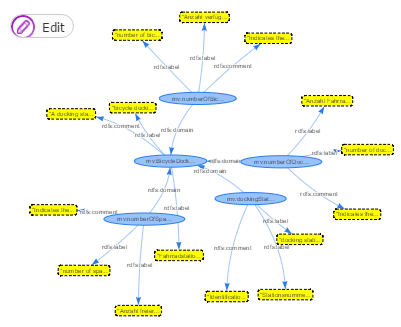
\includegraphics[width=6.7cm]{img/edit_not_clicked.png}}
%  \vspace{1.5cm}
  \centerline{(a) Initial display}\medskip
\end{minipage}
\hfill
\begin{minipage}[b]{0.48\linewidth}
  \centering
  \centerline{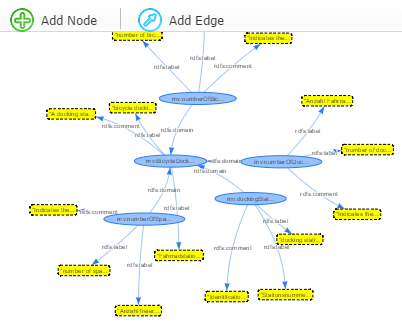
\includegraphics[width=6.7cm]{img/edit_clicked.png}}
%  \vspace{1.5cm}
  \centerline{(b) \textit{Edit} clicked}\medskip
\end{minipage}
\begin{minipage}[b]{\linewidth}
  \centering
  \centerline{
\includegraphics[width=13cm]{img/edit_node_selected.png}}
%  \vspace{1.5cm}
  \centerline{(c) A node is selected}\medskip
\end{minipage}
\hfill
\begin{minipage}[b]{\linewidth}
  \centering
  \centerline{
\includegraphics[width=13cm]{img/edit_edge_selected.png}}
%  \vspace{1.5cm}
  \centerline{(d) An edge is selected}\medskip
\end{minipage}
\begin{minipage}[b]{\linewidth}
  \centering
  \centerline{
\includegraphics[width=13cm]{img/edit_add_node.png}}
%  \vspace{1.5cm}
  \centerline{(e) \textit{Add Node} clicked}\medskip
\end{minipage}
\hfill
\begin{minipage}[b]{\linewidth}
  \centering
  \centerline{
\includegraphics[width=13cm]{img/edit_add_edge.png}}
%  \vspace{1.5cm}
  \centerline{(f) \textit{Add Edge} clicked}\medskip
\end{minipage}
%
\caption{Different states of the graphical manipulation toolbar, depending on the user interaction with the graphical interface.}
\label{img:toolbar}
%
\end{figure}


\subsection {Synchronization}
\label {subsec:synchronization}

The synchronization module was designed to keep both editors updated, meaning that the changes in one view are automatically reflected in the other view, without user interaction. The updates are made only if the modifications pass certain rules of correctness, as a measure to prevent the propagation of errors between the two editors.

The implementation of this functionality took off from the idea of maintaining an underlying model as a common representation for the content of each editor. The logic always keeps two versions of the model: the new one, created when one view is modified and the changes are not yet reflected in the other view, and the one before, when both editors were consistent with the model. As a result, when textual changes are detected, the new model is constructed and a comparison with its older version is performed. In case any changes are detected, they will be transmitted to the graphical view. Similarly, the visual modifications are used to build a new model which will be further turned into text. \autoref{img:sync_process} displays the general synchronization process. In what follows, we will describe in detail how the changes propagation occurs on each side.

\begin{figure}[!htbp]
	\centering
  	\centerline{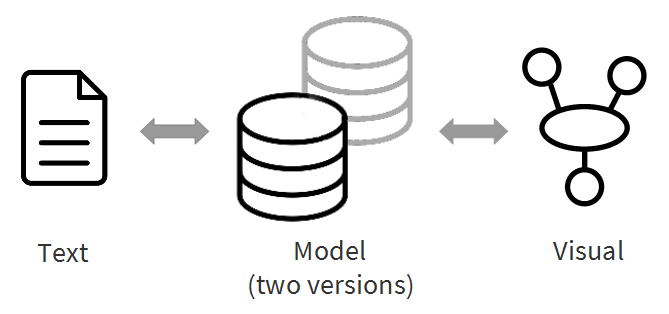
\includegraphics[width=.7\linewidth]{img/sync_process.png}}
	\caption{A broad view of the synchronization process.}
	\label{img:sync_process}
\end{figure}

As mentioned in \nameref{sec:preliminaries}, the code editor is managed by the \textit{Codemirror} library. Changes detection is handled by this library, which triggers an event every time the editor content is modified. The propagation of these changes towards the model relies on the parsing functionality offered by the \textit{N3.js} library. With each change event, the Turtle code is parsed and in case the new version is syntactically valid, the triples that were found are returned. Then, these triples are fetched in order to be stored into an array that will play the role of the underlying model. A triple is basically a Javascript object with three fields (``subject'', ``predicate'' and ``object''), where the value of each field is a string representing the URI of an entity.

\begin{figure}[!htbp]
	\centering
  	\centerline{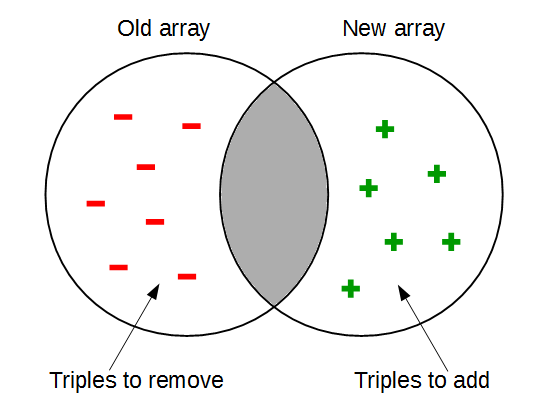
\includegraphics[width=.62\linewidth]{img/array_diff.png}}
	\caption{Symmetrical difference of the old and new array of triples.}
	\label{img:array_diff}
\end{figure}

In order to send the changes to the graphical view, we need to compare the array obtained at the parsing step with its older version ( the one before these changes were performed). For this, a symmetrical difference is calculated between the two arrays (see \autoref{img:array_diff}). The triples that are in the old array but not in the new one will be removed and, accordingly, the triples that are in the new array but not in the old one will be added. An observation to be made here is that there can be three types of changes occurring in the code: insert, update and delete. A special case is the \textit{update}, which will be treated as a composite operation of a delete followed by an insert. Therefore, the triples that were updated will be first removed from the graph and then added with the new values. An update process basically means changing the URI of an entity and since the URIs actually represent the node ids in the network, they cannot be modified. Therefore, in order to keep the consistency between a node's id and its label (which is usually its URI in prefixed form), we considered necessary to remove the nodes that had their URI modified and re-add them with another id represented by the new value.

When updating the graphical view due to textual changes, a set of rules are involved, depending on the operation that is being executed:

\begin{enumerate}
	\item Removing triples:
	\begin{itemize}
		\item subjects and objects (represented by nodes) are removed only if they have exactly one edge or if they are disconnected from the graph (no edge)
		\item predicates (represented by edges) are always removed
	\end{itemize}
	\item Adding triples:
	\begin{itemize}
		\item subjects and objects are added only if they do not exist already
		\item predicates are always added (the array cannot contain duplicate triples)
	\end{itemize}
\end{enumerate}

The inverse synchronization (from visual to text) is triggered every time the user changes the structure of the network. Depending on the modification, different operations (insert, update, delete) are executed on the model, represented by the array of triples. The result is a new version of the model that needs to be further translated into Turtle code. This operation is handled by the \textit{N3.js} library, which features a \textit{Writer} object that serializes one or more triples (given as an array) into an RDF document, where the default format is Turtle. One observation is that the triples are written in the order they are stored in the model so, for keeping the code view consistent, the triples' order must be preserved within the array.

Below, we will explain how pushing changes into the model works in the case of each graphical modification:

\begin{enumerate}
	\item Creating a node - the node is inserted graphically into the network but no updates occur on the model as the node has no edges yet, therefore it forms no triples. Due to the lack of a reasonable representation in the code of a node that is disconnected, we considered that the best approach, in this case, is to make this element known to the code view as soon as it gets linked to another node. Regarding the label of a new node, it will be shown as the short version of its URI (with shrinked prefix) if any abbreviation is provided. If the value is given in short version but without a prefix, the base prefix will be prepended, if any available in code. Otherwise, the label will be shown as introduced by the user. If the label exceeds 15 characters though, the text is truncated and the complete value will be available as a tooltip.
	\item Creating an edge -  linking two nodes through a new edge is equivalent to creating a new triple. Depending on the direction of the edge, the type of each of the two nodes can be determined. The convention is that at the base of the arrow is the subject and at the tip - the object. Drawing an edge from a literal is prohibited through an error alert, as literals can never be subjects. Once we have determined the elements of the triple, we can insert it into the model. In order to avoid having the same subject appear multiple times in the code, and thus preserve the Turtle layout, we considered the following: when inserting a new triple into the array, we search for the last triple having the same subject and we introduce the new one exactly after it. If no such triple was found, the new value is inserted at the end of the array and, therefore, it will appear at the end of the code view.
	\item Editing a node or an edge - this operation refers to the modification of an entity's URI. The triple in which it is contained is searched in the model and, depending on its type (subject, predicate or object), the corresponding field of the triple receives the new value (the existing URI string is replaced with the given one).
	\item Deleting a node - when a node is removed, its edges also disappear from the network. As an edge defines a triple, the number of triples to be removed from the model is equivalent to the number of edges that get deleted together with the node. After these triples are identified and the model is updated, the result is that the code view will erase all triples containing the deleted node as a subject or an object.
	\item Deleting an edge - this is equivalent to removing exactly one triple, therefore one element gets erased from the array.
\end{enumerate}

Some of the operations performed on the array of triples can be quite expensive when the graph is large (thousands of nodes and edges). The symmetrical difference, in particular, can reach a quadratic complexity. In order to improve the time performance, we considered other data structures for storing the triples. Since each triple in the model is unique, we thought of using sets. After performing some operations on this data structure with triple objects, we concluded that the costs vary to a very low extent so we decided to continue working with arrays due to their ease of use in Javascript. The only difference was made by structures that are optimized to work with RDF data as triple arrays. One such object is offered by the \textit{N3.js} library. It is called a \textit{store} and it allows storing triples in memory and finding them fast. The downsides are that it does not allow inserting a triple at a certain index and it does not preserve the triples order as they are parsed from the code. As a compromise, we decided to use stores only for calculating the symmetrical difference and continue performing the other operations on arrays.

In order to easily track the results of the synchronization operations presented above, the two editors need to be simultaneously visible. Initially, we followed the interface layout offered by TurtleEditor (an example can be found in \cite{Petersen2016}) and we created a tabbed view so that the user can switch between the two editors. \autoref{img:tabbed_view} shows the user interface when each of the tabs are active.

\begin{figure}[!htbp]
	\begin{minipage}[b]{\linewidth}
 	 	\centering
  		\centerline{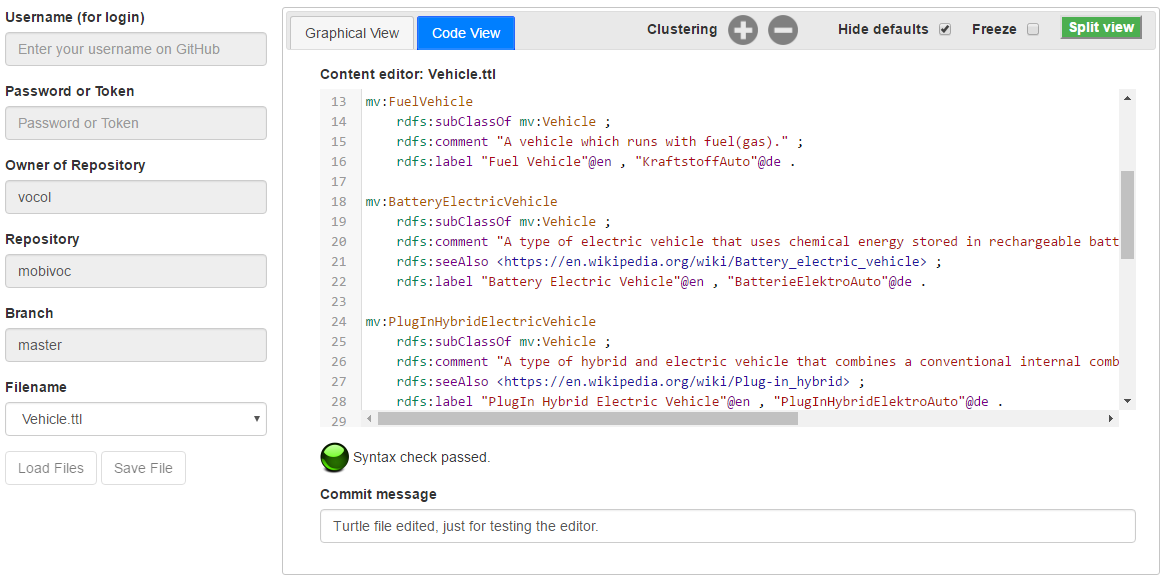
\includegraphics[width=\linewidth]{img/code_view.png}}
  		\centerline{(a) Code view}\medskip
  		%\vspace{1cm}
	\end{minipage}
	\hfill
	\begin{minipage}[b]{\linewidth}
 		 \centering
  		\centerline{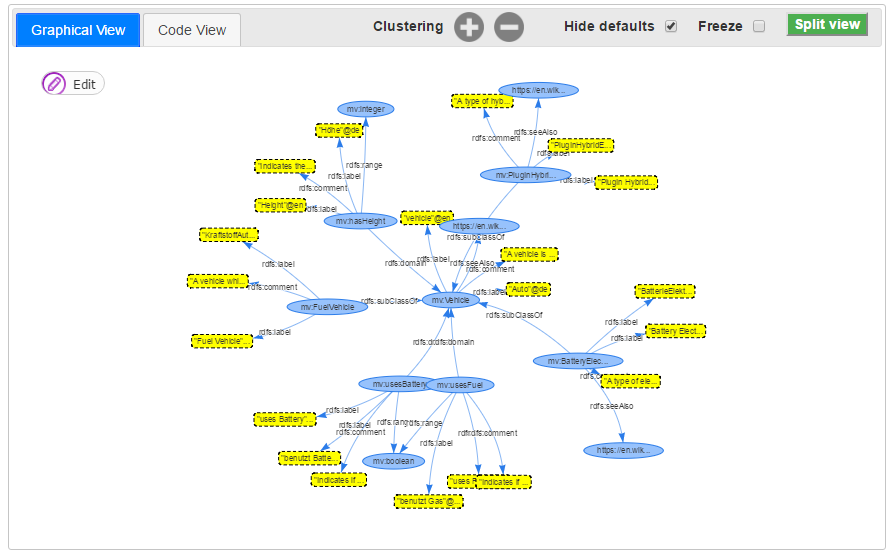
\includegraphics[width=\linewidth]{img/graphical_view.png}}
		%\vspace{1.5cm}
  		\centerline{(b) Graphical view}\medskip
	\end{minipage}
\caption{Graphical user interface of the two editors in tabbed view.}
\label{img:tabbed_view}
\end{figure}

Since the synchronization operates instantly, the user should be able to supervise changes in both views in parallel. Therefore, we also implemented a split view that can be activated through the green button placed on the top right corner of the tabbed view. This removes the left side containing the forms needed for GitHub interaction and puts together the views that were previously accessible only in tabs. The editors are separated by a movable bar so each view can be extended in width as much as the screen allows. In order to go back to the tabbed view, a green button is available on the top right corner, as shown in \autoref{img:split_view}. The splitting functionality is handled by the \textit{spli-pane.js} library\footnote{\url{https://github.com/shagstrom/split-pane}}, which looks for HTML containers having set a certain CSS class that defines them as components of the view.

Another feature available in the split view is term highlighting. When a node is selected in the graphical view, the effect is that all of its occurrences in the code are marked with a light-green background. In addition, the text editor updates its view so that the first line where the entity appears can be visible. Moreover, the highlights are available on the scrollbar as well, enabling the user to easily navigate between multiple occurrences of a term (see \autoref{img:split_view}).This functionality is implemented as follows: when the user clicks on a node in the network, an event is triggered and data regarding the selected entity is passed to a handler function. Then, the label of the entity is searched within the code using pattern matching and the corresponding pieces of text are marked employing some of the functionalities offered by \textit{Codemirror}. The highlights on the scrollbar are implemented using the same library with one of its add-ons - \textit{matchesonscrollbar.js}.

\begin{landscape}
\begin{figure}[ht]
\centering
    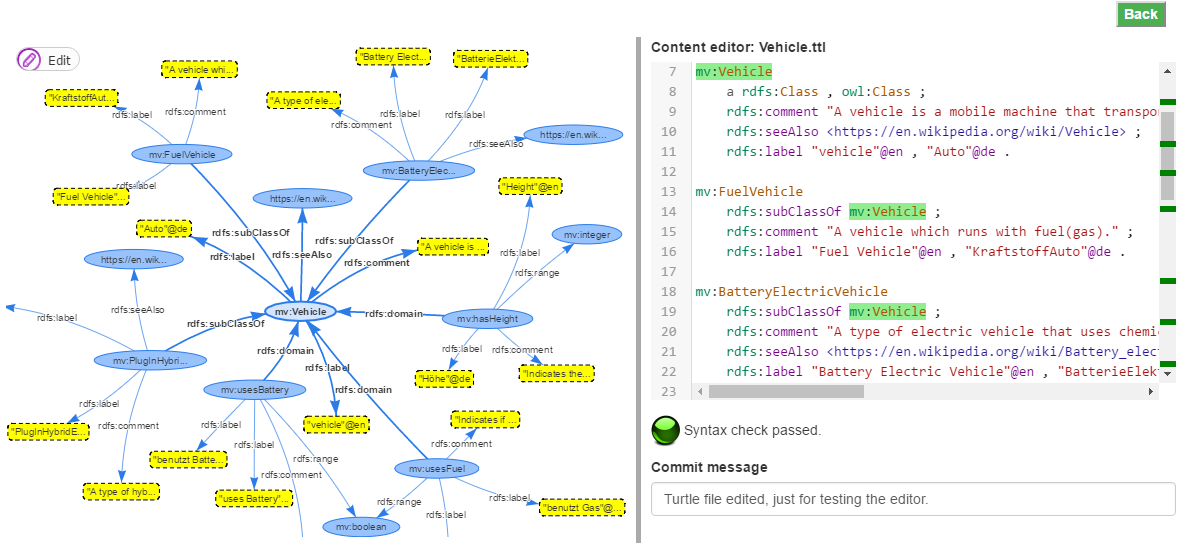
\includegraphics[width = 20cm]{img/split_view.png}
    \vspace{1.2cm}
    \caption{Graphical user interface of the split view.}
    \label{img:split_view}
\end{figure}
\end{landscape}


\subsection {Visualization}
\label{subsec:visualization}

The visualization of RDF data can become a quite complex task when dealing with large vocabularies. Certain techniques need to be employed in order to keep the interaction with the graphical editor usable and intuitive. Part of this task has been taken care of by the \textit{vis.js} library, through its \textit{layout} and \textit{physics} modules.

The \textit{layout} module governs the initial and the hierarchical positioning. We chose to keep its default values: non-hierarchical, using the Kamada Kawai algorithm \cite{Kamada1989} for the initial layout. As a result, the graph elements are positioned in a symmetrical way so that the edges have approximately the same length and there are as few crossings as possible between them.

The \textit{physics} module is concerned with the moving simulation and also with the graph stabilization, by forcing the nodes to always return to their precomputed positions, based on certain parameters. The positions are calculated using the Barnes-Hut algorithm \cite{Barnes1986}, which according to the \textit{vis.js} documentation\footnote{\url{http://visjs.org/docs/network/physics.html}}, is ``the fastest and recommended solver for non-hierarchical layouts''. It is a quadtree based gravity model which groups together bodies that are close enough. We modified the default values of the following parameters in order to speed up the drawing of large graphs:

\begin{itemize}
	\item gravitational constant: -2500; a negative value refers to repulsion, where the lower the value, the higher the repulsion; we decreased the gravity from its default value (-2000) in order to obtain a better visibility for large graphs.
	\item spring constant: 0.001; the edges are modeled as springs, where the constant refers to how ``robust'' the spring is; this value will determine the edges to be more ``loose'' (than the default value, 0.04), also for visibility purposes.
	\item spring length: 50; it refers to the length of the spring in resting state; we decreased it from the default value (95) is order to avoid a too wide spread of the graph into space.
\end{itemize}

The last two parameters in conjunction with the continuous smoothing of the edges (see \autoref{subsec:graphical_editing}) turn out to give good results in the case of large graphs, with respect to time performance and aesthetics.

The physics functionalities prove to be useful when it comes to an intuitive interaction with the graph. However, they represent additional overhead for the time performance and even burden the navigation of large graphs by generating lag and slow movements. Moreover, the user might want to manually rearrange the graph layout and drag the nodes at certain positions, without having them automatically rearranged by the physics engine. We enabled this possibility by providing a ``Freeze'' checkbox which is by default unchecked, meaning that the physics laws are active. This feature is available in tabbed view, as shown in \autoref{img:tabbed_view}. For a close-up, please check \autoref{img:visualization_buttons}. This is achieved by setting the ``enabled'' flag of the physics module to false. 

\begin{figure}[htb]
	\centering
	\vspace{.5cm}
  	\centerline{
\includegraphics[width=0.95\linewidth]{img/visualization_buttons.png}}
	\caption{Functions of the visualization module.}
	\label{img:visualization_buttons}
\end{figure}

Another function available in the visualization configurator is called ``Hide defaults''. This comes as a fulfillment of one of the requirements stating that the user should be able to hide the nodes that are highly connected and, so, generating a lot of clutter. We chose the ``defaults'' to be all the entities that are part of the \textit{RDF}, \textit{RDFS} and \textit{OWL} namespaces and we made this clear to the user by providing a tooltip. The functionality is implicitly enabled when the page is loaded and, in order to show all the nodes, the user has to uncheck it (see \autoref{img:visualization_buttons}). When the checkbox is ticked, the default nodes are not removed from the graph, they are just hidden. This is achieved through the \textit{nodes} module, which features a ``hidden'' flag for each node in the dataset. We filter the nodes by their URI and then we set this flag to true on the result set. Also, an event has to be triggered in order to have the network redrawn and commit the updates. The effect of applying this option is shown in \autoref{img:defaults}, where we provided two examples: one quite small graph (33 triples) and one large graph (1573 triples), where the nodes are clustered. As it can be observed, even for small graphs this is useful, as it makes it more clear to see the nodes that are part of the defined vocabulary. For large graphs, hiding these nodes comes as a necessity, as it is extremely cumbersome to distinguish anything among the large number of edges.

\begin{figure}[htb]
\begin{minipage}[b]{.48\linewidth}
  \centering
  \centerline{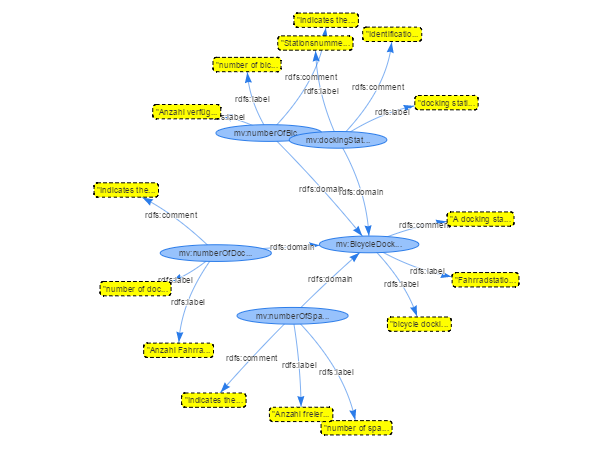
\includegraphics[width=6.7cm]{img/no_defaults.png}}
  \centerline{(a) Small graph, no defaults}\medskip
  \vspace{.5cm}
\end{minipage}
\hfill
\begin{minipage}[b]{0.48\linewidth}
  \centering
  \centerline{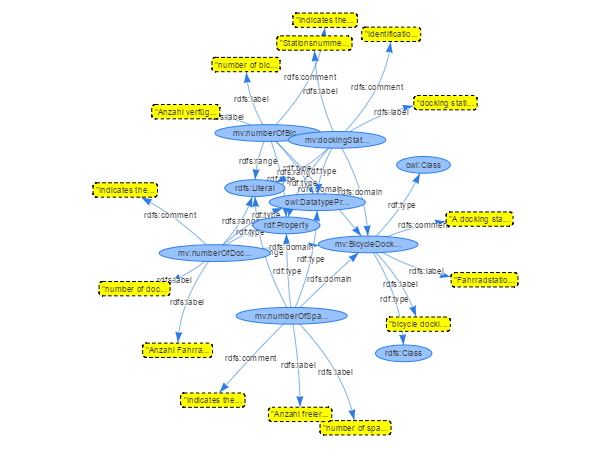
\includegraphics[width=6.7cm]{img/with_defaults.png}}
  \centerline{(b) Small graph with defaults}\medskip
  \vspace{.5cm}
\end{minipage}
\begin{minipage}[b]{0.48\linewidth}
\centering
  \centerline{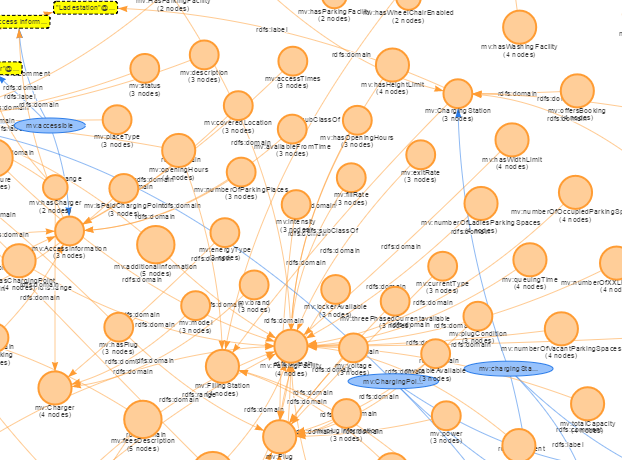
\includegraphics[width=6.7cm]{img/no_defaults1.png}}
  \centerline{(c) Large graph, no defaults}\medskip
\end{minipage}
\hfill
\begin{minipage}[b]{0.48\linewidth}
  \centering
  \centerline{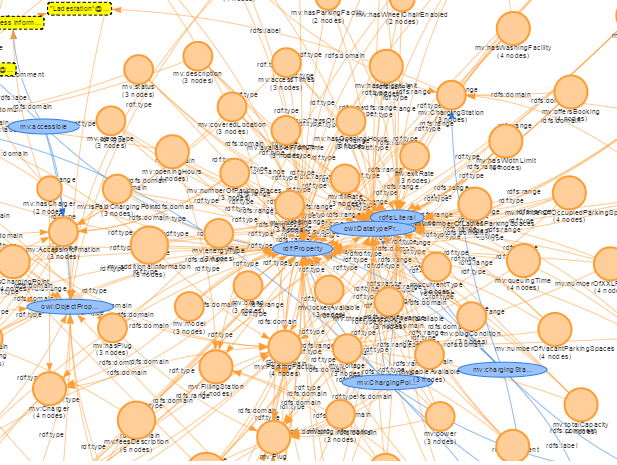
\includegraphics[width=6.7cm]{img/with_defaults1.png}}
  \centerline{(d) Large graph with defaults}\medskip
\end{minipage}
\caption{Hiding and showing nodes from the default namespaces on two different sized graphs.}
\label{img:defaults}
\end{figure}

The last and most important functionality in the visualization module is clustering. Its implementation came as a requirement for improving both the interaction with large graphs (over 500 nodes) and the time performance when any graphical operation is involved. \textit{vis.js} comes with support for clustering, offering different methods for grouping nodes together based on certain properties. Out of these, we chose clustering outliers, where an outlier represents a node with exactly one edge , i.e., one neighbor. The method basically groups together these nodes with their respective connected node and it can be called as long as there are still outliers in the graph, meaning that clusters can be joined together with other clusters. The graphical result of this process is that the outlier nodes will disappear from the graph, being replaced by another node which encapsulates them and plays the role of the cluster. This type of nodes can be differentiated through a set of properties:

\begin{itemize}
	\item shape: circle.
	\item color: light orange with a darker shade for the border.
	\item label: composed of two lines, where the first line is the label of the common neighbor node for each outlier and the second line represents the number of nodes that are contained within the cluster; when two clusters are joined together, the number of children belonging to each one of them is summed. The label is displayed outside the dot shape (as opposed to normal nodes) because, by design, when the label is inside, the length of the text determines the size of the node. When it is placed outside, then the size can be calculated using different criteria.
	\item size: depends on the number of children and it grows linearly.
	\item repulsion: increases linearly with the size.
\end{itemize}

The clustering process can be manipulated using the plus and minus buttons available in the tabbed view (see \autoref{img:visualization_buttons}). The plus sign clusters any outliers currently existing in the graph, be they normal nodes or already clusters. This process can be repeated as long as there are still outliers in the network. With each repetition, one more level of clustering is added. In order to open the clusters, the minus sign can be used. The nodes will be declustered with respect to their levels, so it may be possible that the minus needs to be clicked multiple times in order to reach the state where there are no more clusters in the graph. Clicking a cluster node also removes one clustering level, the effect being that the node is opened up and the hidden graph elements inside it are set free. \autoref{img:clusters} shows the effect of applying two clustering levels on a graph consisting of 370 triples. Please note that pressing the plus button one more time would have no effect, even though in (c) it seems like there are still outliers in the graph. This is because the default nodes are hidden but they are still part of the graph, maintaining connections with other nodes. After displaying them in (d), we see that there are actually no more outliers and this is the reason why the clustering stopped after two levels.  

The clustering process is mainly handled by the \textit{vis.js} library. We only needed to take care of the list of currently existing clusters by managing the insertions and deletions that come with every cluster level. Also, the cluster node properties presented above are set manually as we needed to override the default values in order to suit our needs with respect to intuitiveness.

One last observation needs to be made with respect to the number of clustering levels that are pre-applied when a network is initially drawn. This happens when a file is loaded in the Turtle editor or when code is pasted in the text view. Small graphs (below 500 triples) are displayed unclustered, while graphs consisting of over 500 and 1000 triples have applied one and, respectively, two clustering levels. This is done primarily for reducing the time used for the initial drawing of the network, but also for better visibility and navigation through the graph.

\begin{figure}[htb]
\begin{minipage}[b]{.48\linewidth}
  \centering
  \centerline{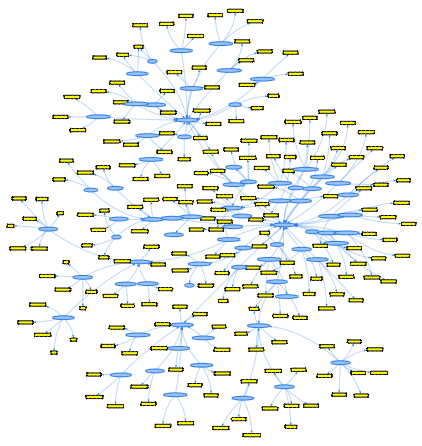
\includegraphics[width=6.7cm]{img/cluster0.png}}
  \centerline{(a) No clusters}\medskip
  \vspace{.5cm}
\end{minipage}
\hfill
\begin{minipage}[b]{0.48\linewidth}
  \centering
  \centerline{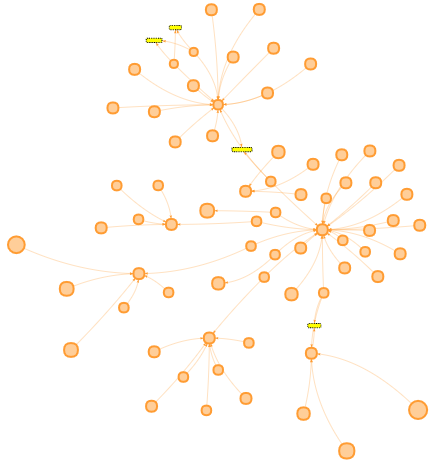
\includegraphics[width=6.7cm]{img/cluster1.png}}
  \centerline{(b) Level 1}\medskip
  \vspace{.5cm}
\end{minipage}
\begin{minipage}[b]{0.48\linewidth}
\centering
  \centerline{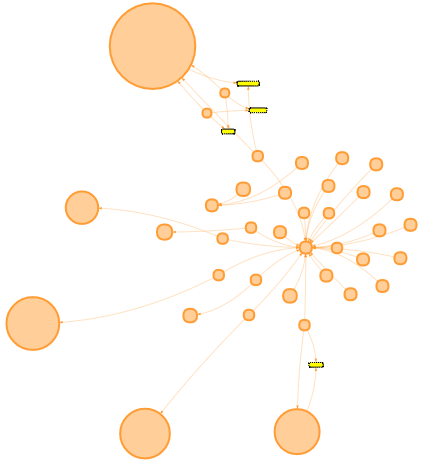
\includegraphics[width=6.7cm]{img/cluster2.png}}
  \centerline{(c) Level 2}\medskip
\end{minipage}
\hfill
\begin{minipage}[b]{0.48\linewidth}
  \centering
  \centerline{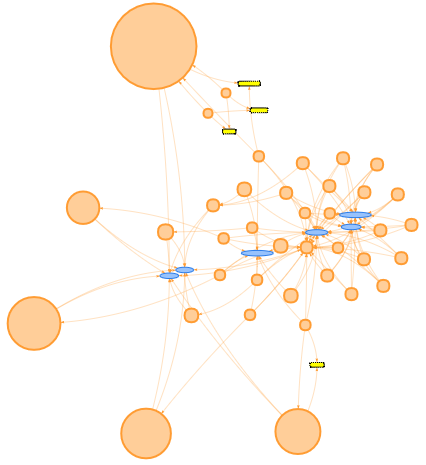
\includegraphics[width=6.7cm]{img/cluster2_with_defaults.png}}
  \centerline{(d) Level 2, defaults displayed}\medskip
\end{minipage}
\caption{Applying the maximum levels of clustering on a graph consisting of 370 triples.}
\label{img:clusters}
\end{figure}











